\chapter{Introduction}
\section{Characteristics of a flow sensor}

There are 2 types of moving media \cite{handbook}:
\begin{itemize}
	\item liquids. \textit{Ex:} water, oil, gasoline.
	\item air and gas. \textit{Ex:} \ce{O2}, \ce{N2}, \ce{CO2}, \ce{CH4}.	
\end{itemize}

Although flow sensors may be simple as detecting velocity of the fluid or air/gas, 
\section{Several examples of flow sensors}
\subsection{Pressure gradient technique}
This technique is applicable only for measuring \textbf{steady flow of nonviscous, incompressible medium} using Bernoulli equation, which relates to \textit{flow resistance}. The working principle of this technique is as follows:
\begin{enumerate}
	\item Create a medium impeding the flow motion in a section of the pipe, such as orifices, porous plugs, and Venturi tubes.
	\item Place 1 differential pressure sensor between the normal sections or 2 absolute pressure sensors in each normal section of the pipe.
	\item Because the high resistance area creates a slight pressure difference in the flow, the mass transferred through the pipe can be estimated.
\end{enumerate}
\begin{figure}[ht]
	\centering
	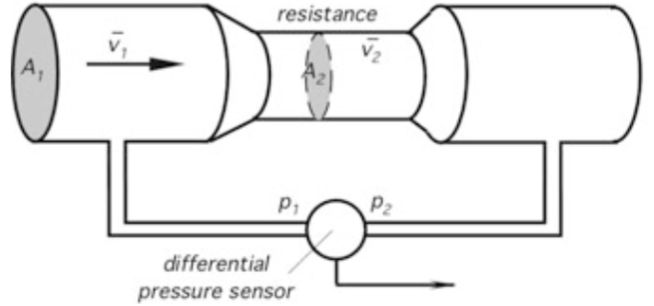
\includegraphics{pressure gradient}
	\caption{Pressure gradient technique example using narrow channel flow. Small cross section causes }
	\label{fig:01}
\end{figure}

The equation for finding mass flow is:
\begin{equation}
q = \epsilon A_2 \sqrt{\Delta p}
\end{equation}

where
\begin{itemize}
	\item $ q $ is the mass flow per unit time,$ \unit{kg/s} $.
	\item $ \epsilon $ is the calibration coefficient.
	\item $ A_2 $ is the cross section of the high resistance area,$ \unit{m^2} $.
	\item $ \Delta p$ is the pressure difference,$\unit{Pa} $.
\end{itemize}

Derivation of the equation is provided in chapter 12 \cite{handbook}.

Advantage of the pressure gradient method is in the absence of moving components and use of standard pressure sensors that are readily available. A disadvantage is in the restriction of flow by a resistive device.

\subsection{Thermal transport sensors}
